\pdfminorversion=4
\PassOptionsToPackage{x11names}{xcolor}
\documentclass{beamer}
%\documentclass[handout]{beamer}
%\usepackage{handoutWithNotes}
%\pgfpagesuselayout{4 on 1 with notes}[a4paper, border shrink=5mm]
%% Method from https://github.com/gdiepen/latexbeamer-handoutWithNotes
\usepackage{subcaption}
\usepackage{appendixnumberbeamer}
\usepackage{grffile}
\usepackage[utf8]{inputenc}
%\usepackage[hang,flushmargin]{footmisc}

\usepackage{tikz}
\usetikzlibrary{shapes.geometric, arrows, positioning}

\usepackage[style=authortitle,backend=biber]{biblatex}
\addbibresource{refs.bib}

\usetheme{Sheffield}
\useinnertheme{SheffieldCBM}

\addbibresource{library.bib}

\newsavebox{\foobox}
\newcommand{\slantbox}[2][0]{\mbox{%
        \sbox{\foobox}{#2}%
        \hskip\wd\foobox
        \pdfsave
        \pdfsetmatrix{1 0 #1 1}%
        \llap{\usebox{\foobox}}%
        \pdfrestore
}}
\newcommand\unslant[2][-.25]{\slantbox[#1]{$#2$}}

%  \item specially for beamer
\renewcommand{\footnotesize}{\scriptsize}

\tikzset{
    userblock/.style={
    rectangle,
    rounded corners,
    minimum width=3cm,
    minimum height=1cm,
    align = center,
    draw=shefblue,
    line width = 1pt,
  },
  flowblock/.style={
    rectangle,
    rounded corners,
    minimum width=3cm,
    minimum height=1cm,
    align = center,
    draw=sgreylight,
    line width = 1pt,
  },
  arrow/.style={
    line width = 1.5pt,
    ->,
    > = stealth,
    draw=shefblue,
    },
  dashdouble/.style={
    line width = 1.5pt,
    <->,
    > = stealth,
    draw=shefblue!70,
    },
  dashbend/.style={
    line width = 1.5pt,
    ->,
    > = stealth,
    draw=shefblue!70,
    bend right=20,
    },
}

\newenvironment<>{varblock}[2][.9\textwidth]{%
  \setlength{\textwidth}{#1}
  \begin{actionenv}#3%
    \def\insertblocktitle{#2}%
    \par%
    \usebeamertemplate{block begin}%
}{%
  \par%
    \usebeamertemplate{block end}%
  \end{actionenv}%
}

\begin{document}

\title{Software Sustainability}
\subtitle{The why and the how}
\author[Phil Tooley - Sheffield]{Phil Tooley\\University of Sheffield}
\date[CFM:SIG 20/09/2018]{Cardiovascular Fluids Modelling SIG\\20 September 2018}


\begin{frame}
\maketitle
\end{frame}

\begin{frame}
  \frametitle{Science relies on research software}
  \begin{block}{2014 UK Research Software Survey\footnotemark}
    \centering
    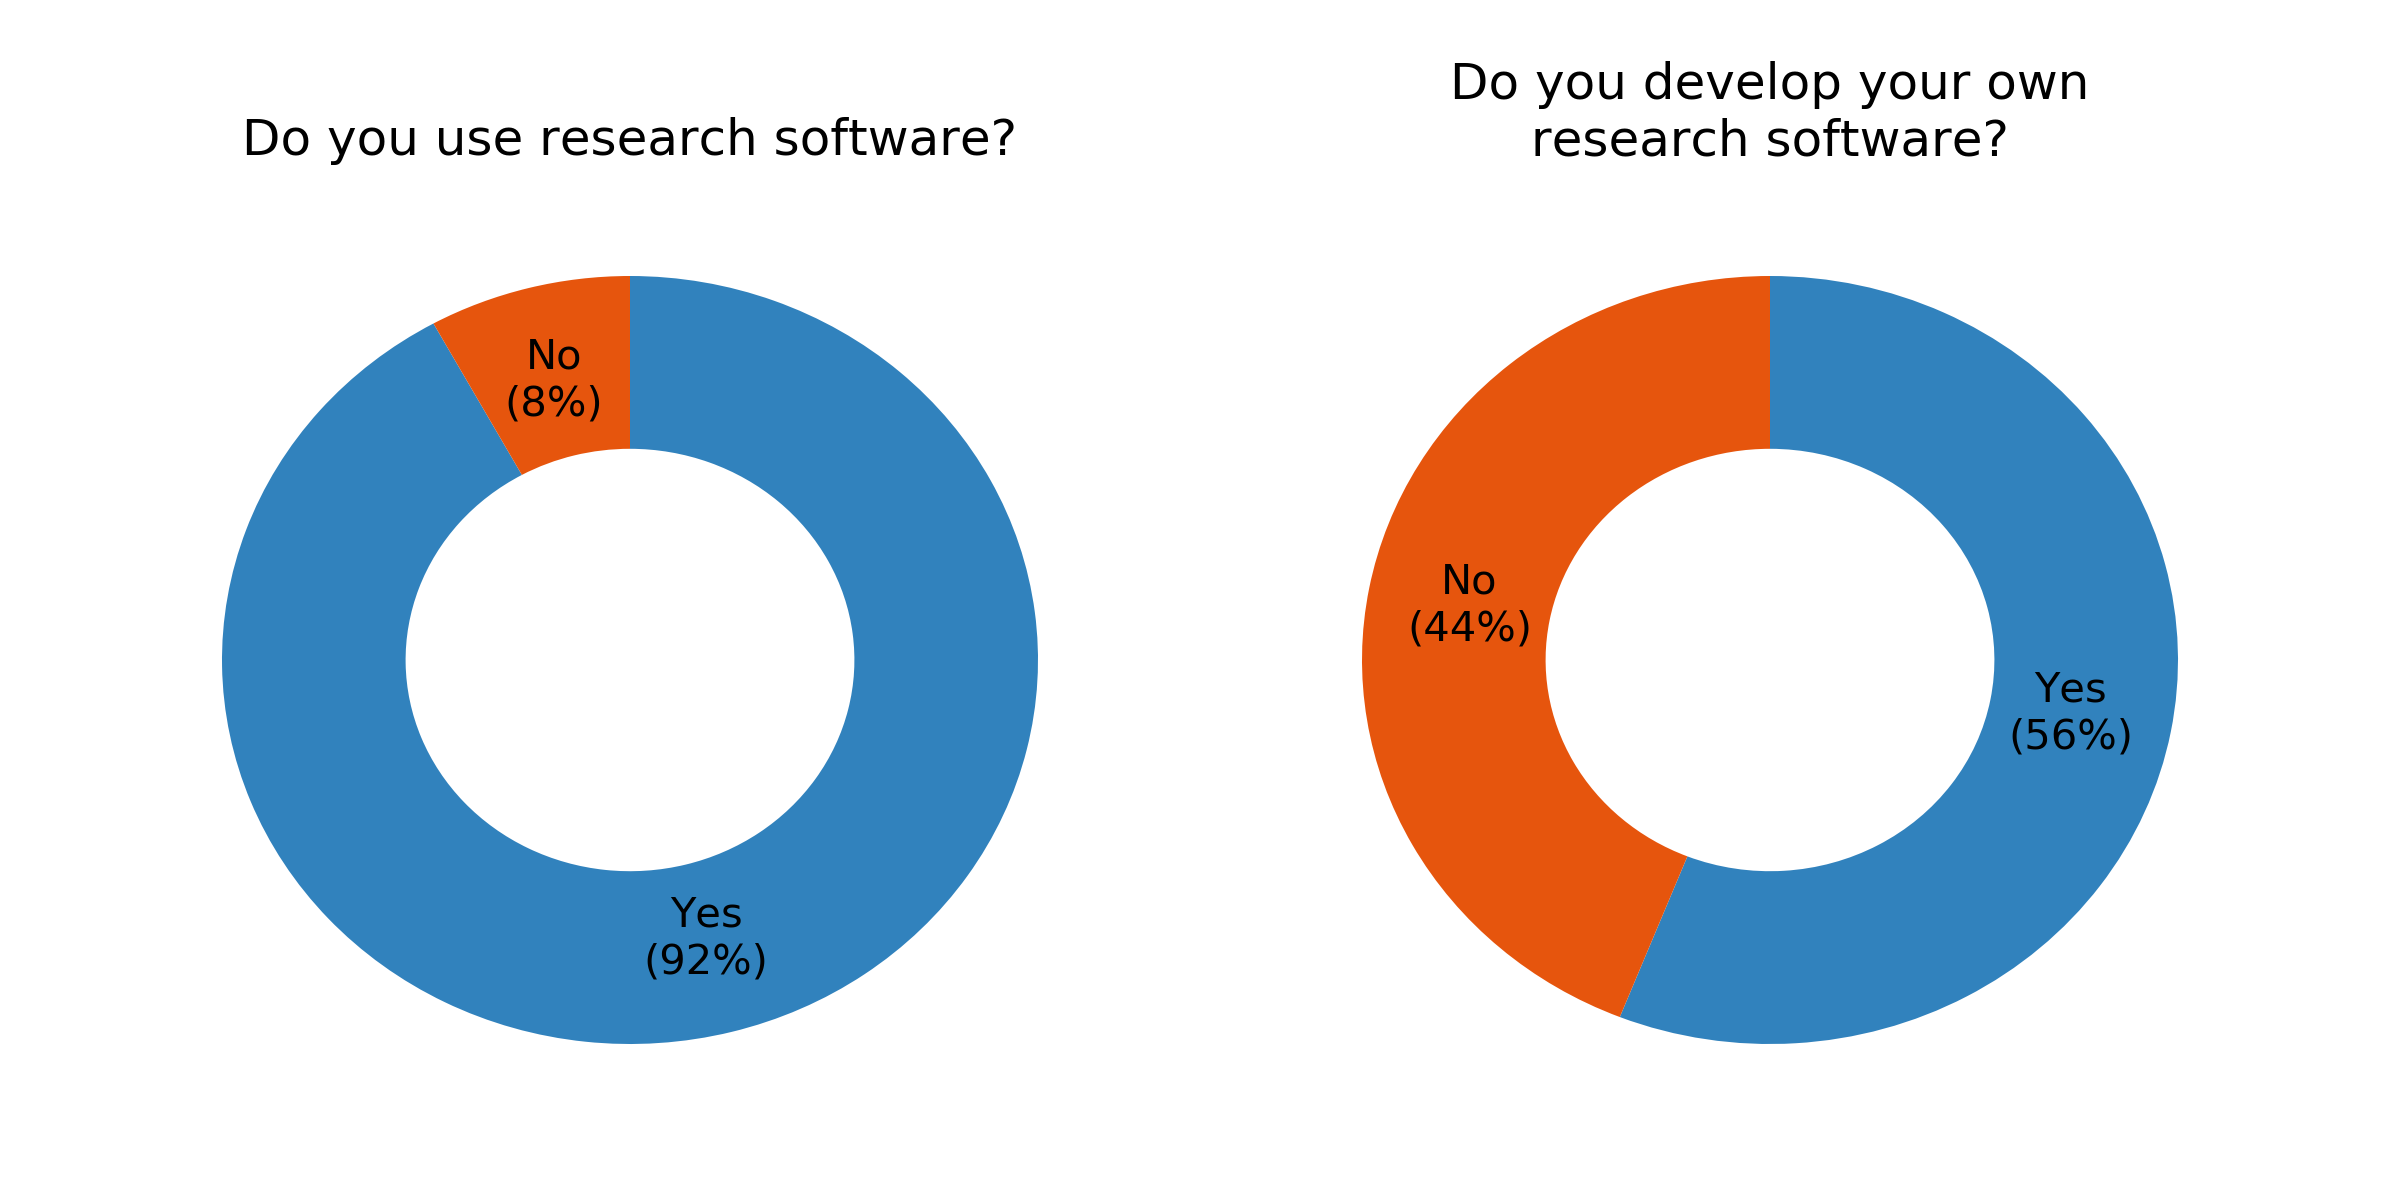
\includegraphics[width=0.9\textwidth]{surveyres.png}
  \end{block}
  \footnotetext[1]{S.J. Hettrick et al, UK Research Software Survey 2014}
\end{frame}

\begin{frame}
  \frametitle{It must be \emph{good} research software}
  \centering
  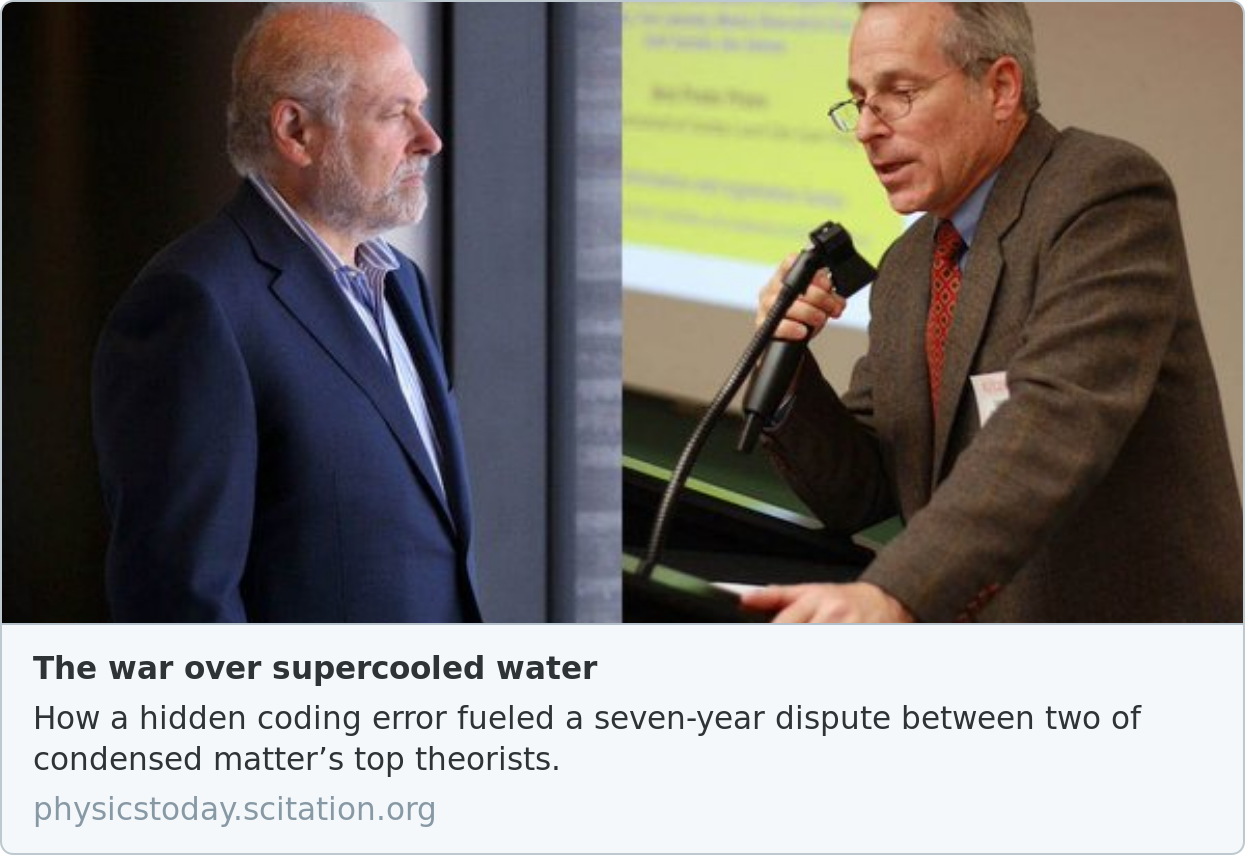
\includegraphics[width=0.8\textwidth]{phystoday_codeerror}
  \let\thefootnote\relax\footnote{Source: Physics Today, DOI:10.1063/PT.6.1.20180822a}
\end{frame}

\begin{frame}
  \frametitle{Recognising the Problem}
  \begin{block}{Software Sustainability Institute\footnotemark[2]}
    \begin{itemize}
      \item Funded in 2010 by EPSRC to promote sustainable development of research software and now
        a collaborative effort by multiple research councils
      \item Provide training and support for developers of scientific software
      \item Focus on reproducible research and recognising software as a research output
      \item ``Better software, better research''
    \end{itemize}
  \end{block}
  \vspace{-2em}
  \begin{block}{}
    \raisebox{-0.5\height}{
\includegraphics[width=2cm]{ssi}}
    \hfill
    \raisebox{-0.5\height}{
\includegraphics[width=2cm]{epsrc}}
    \hfill
    \raisebox{-0.5\height}{
\includegraphics[width=2cm]{bbsrc}}
    \hfill
    \raisebox{-0.5\height}{
\includegraphics[width=2cm]{esrc}}
    \hfill
    \raisebox{-0.5\height}{
\includegraphics[width=2cm]{jisc}}
  \end{block}
  \footnotetext[2]{www.software.ac.uk}
\end{frame}

\begin{frame}
  \frametitle{My first research code experience}
  \centering
  \pause
  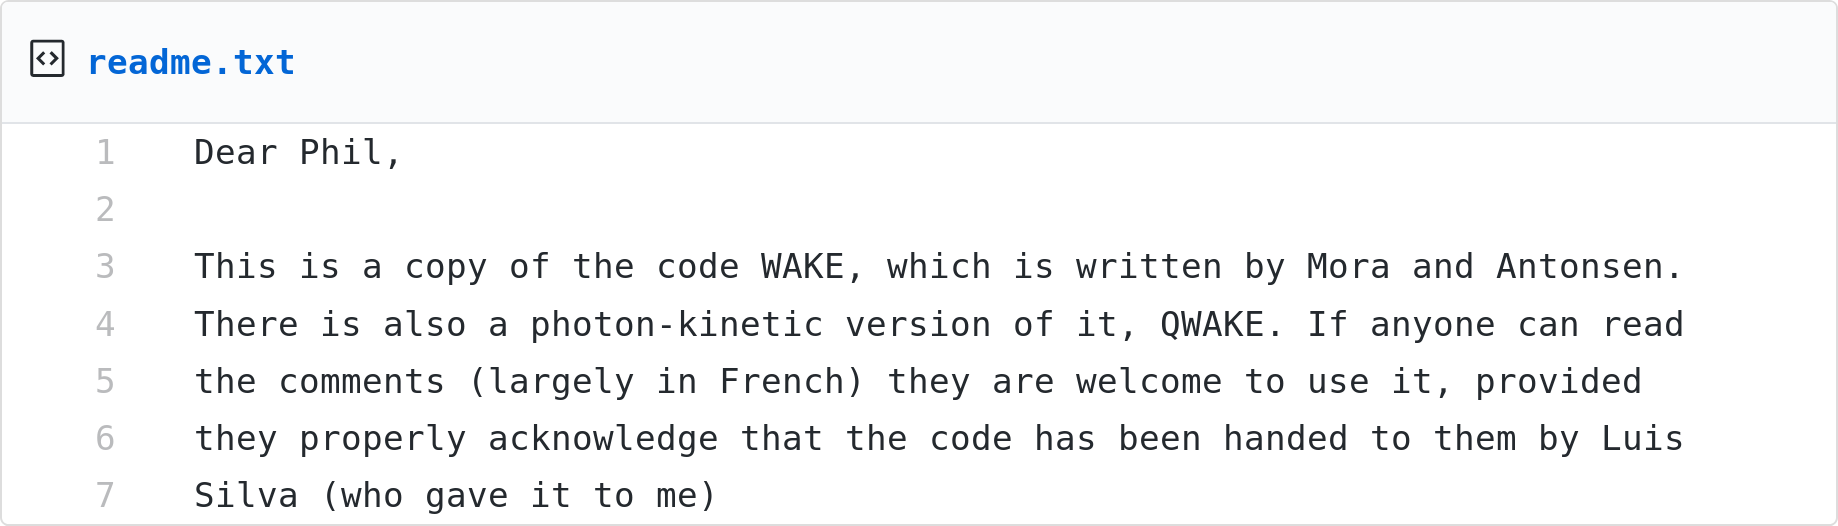
\includegraphics[width=0.9\textwidth]{wakereadme}
  \pause
  \vspace{-1em}
  \begin{block}{}
    \begin{itemize}
      \item[] \alert{How do I run this?}
      \item[] \alert{What will it do?}
      \item[] \alert{How do I interpret the output?}
    \end{itemize}
  \end{block}
\end{frame}

\begin{frame}
  \frametitle{The code I actually used}
  \centering
  \only<1>{
    
\includegraphics[width=0.9\textwidth]{fbpic_readme}
  }
  \only<2>{
    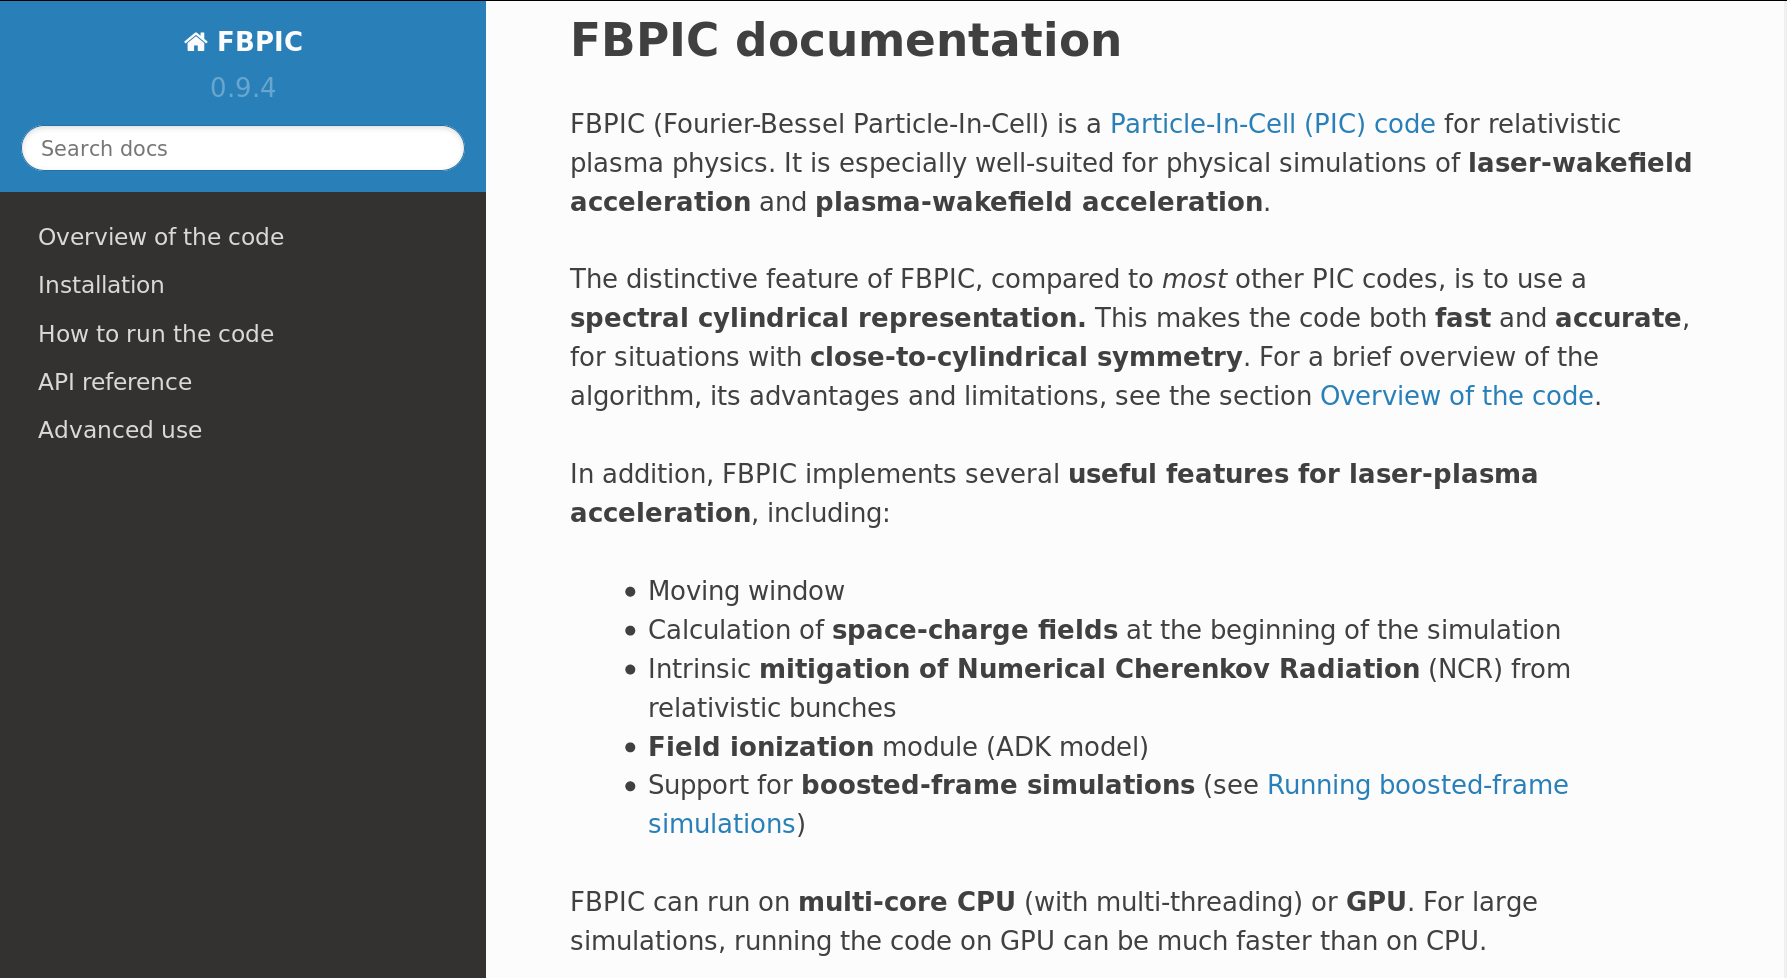
\includegraphics[width=0.9\textwidth]{fbpic_docs}
  }
\end{frame}

\begin{frame}
  \frametitle{Unsustainable Software}
  \begin{columns}
    \begin{column}{0.65\textwidth}
      Symptoms of unsustainable software or development practices include:
      \begin{itemize}
        \item inherited magic/spaghetti code 
        \item versioning hell 
        \item lack of documentation
        \item no tests/benchmarks
        \item custom data formats
        \item hard to modify without breaking
        \item hard to install on new machines
      \end{itemize}
    \end{column}
    \begin{column}{0.35\textwidth}
      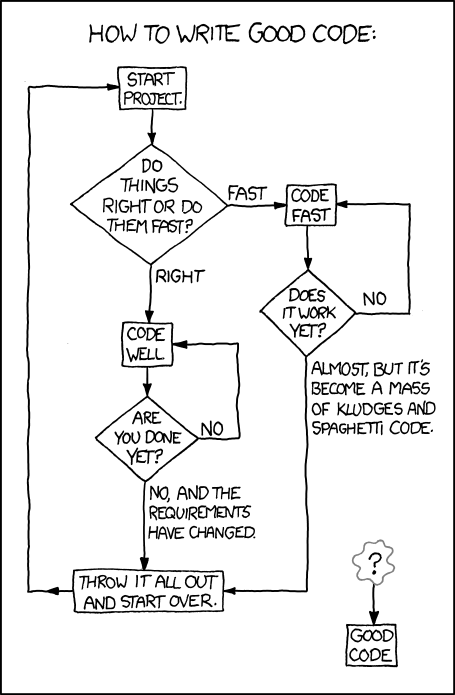
\includegraphics[width=0.8\textwidth]{good_code}
    \end{column}
  \end{columns}
  \vspace{1.5em}
  \pause
  \alert{Writing good software is hard. Maintaining it can be even harder...}
  \let\thefootnote\relax\footnote{Image Source: Randall Munroe, XKCD (https://xkcd.com/844/)}
\end{frame}

\begin{frame}
    \frametitle{How do we make sustainable software?}
    \centering
    \begin{block}{}
      ``\textbf{Software sustainability} describes the practices, both technical and non-technical,
      that allow software to continue to operate as expected in the future. A constant level of
      effort is required to maintain the software's operation.''\footnotemark[3]
    \end{block}
    \begin{block}{Key Considerations}
      \begin{itemize}
        \item Good organisation using version control
        \item Ensuring longevity of software, runnable on new hardware/OSes
        \item Testing and benchmarking to ensure valid results
        \item Documentation - both usage and technical
        \item Dissemination/sharing with wider community
      \end{itemize}
    \end{block}
    \footnotetext[3]{S.J. Hettrick et al., UK Research Software Survey 2014,
    DOI:10.5281/zenodo.1183562}
\end{frame}

\begin{frame}
  \frametitle{Good Code Structure}
  \centering
  \begin{block}{Well structured code is:}
    \begin{itemize}
      \item Easy to understand
      \begin{itemize}
        \item Consistent code style
        \item Names should explain what things do
        \item Use more, simpler, statements
        \item Comments explain design decisions
      \end{itemize}
      \pause
      \item Easy to modify and reuse
      \begin{itemize}
        \item Split up source code into logical units
        \item Use classes to keep variables and their functions together
        \item Keep data and code separate
        \item Don't hardcode variables, use a configuration file
      \end{itemize}
      \pause
      \item Necessary
        \begin{itemize}
          \item Use existing libraries where you can
          \item Don't invent your own data formats
        \end{itemize}
    \end{itemize}
  \end{block}
\end{frame}

\begin{frame}
  \frametitle{Keeping Code Organised}
  \centering
  
\includegraphics[width=0.5\textwidth]{bad_version_control}
\end{frame}

\begin{frame}
  \frametitle{Keeping Code Organised}
  \centering
  \begin{block}{Have you ever}
    \begin{itemize}
      \item Had files with names like ``awesomecode\_v4\_final\_final.py''?
      \item Made a change to code, then wanted to change it back?
      \item Needed to compare two revisions of your code?
      \item Had to maintain different versions of your code?
      \item Wanted to develop code collaboratively?
    \end{itemize}
    \alert{Version control systems exist to help with this}
  \end{block}
\end{frame}

\begin{frame}
  \frametitle{Keeping Code Organised}
  \begin{columns}
    \begin{column}{0.6\textwidth}
      \begin{block}{Version Control Systems (VCS)}
        \begin{itemize}
          \item Keep a full history of changes
          \item Easily restore old versions
          \item<2-> Develop multiple versions together
          \item<2-> Try things out without consequences
          \item<3-> Easily share and collaborate
        \end{itemize}
        \visible<4>{\alert{Most commonly used VCS is git}}
      \end{block}
    \end{column}
    \begin{column}{0.4\textwidth}
      \only<1>{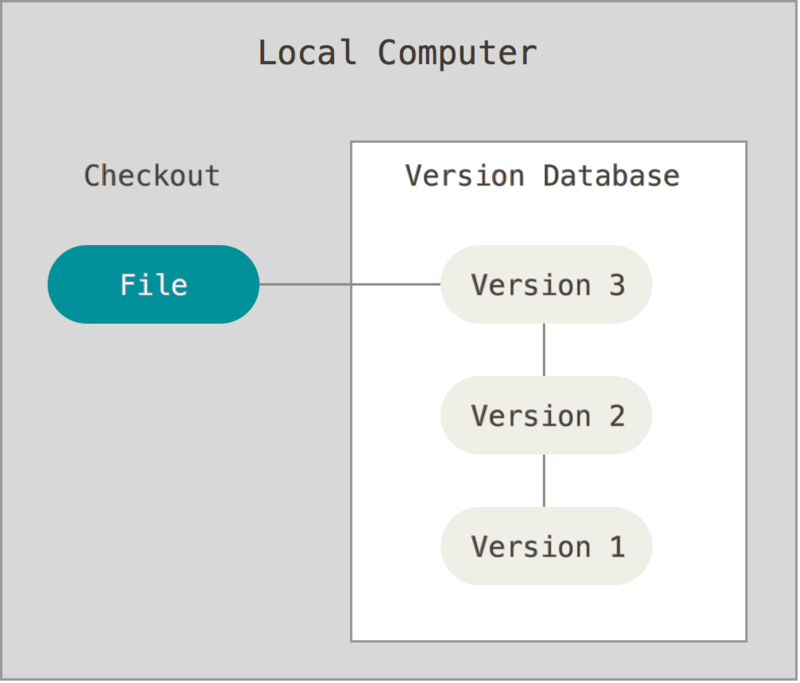
\includegraphics[width=0.9\textwidth]{localvcs}}
      \only<2>{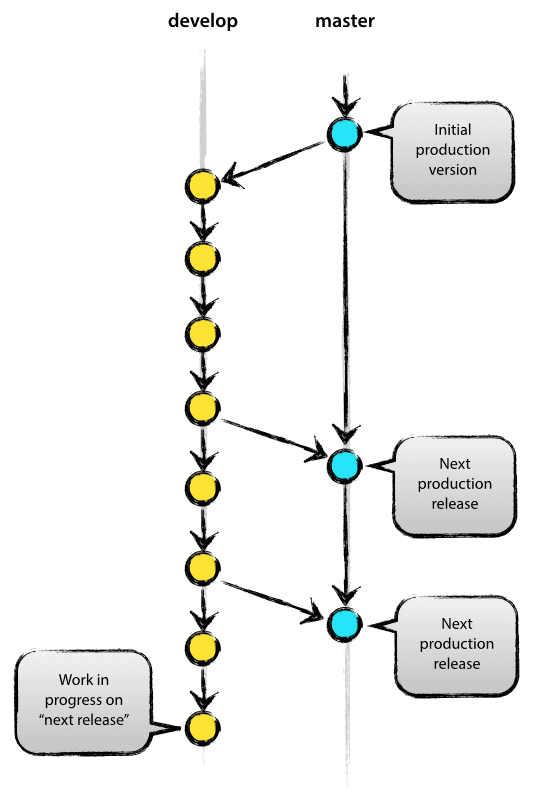
\includegraphics[width=0.75\textwidth]{git-main-branches}}
      \only<3->{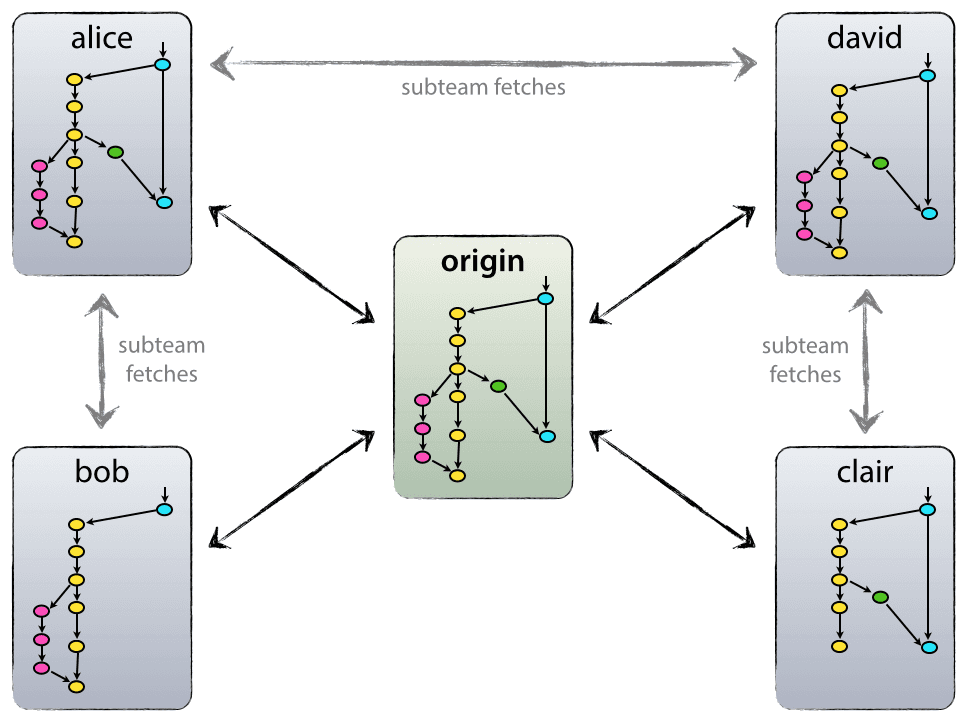
\includegraphics[width=0.9\textwidth]{git-collab}}
    \end{column}
  \end{columns}
\end{frame}

\begin{frame}
  \frametitle{Keeping Code Organised}
  \begin{columns}
    \begin{column}{0.55\textwidth}
      \begin{block}{Github}
        \begin{itemize}
          \item Store your git repositories online
          \item Public repos for open source software development
          \item Free private repos for education and research
          \item Community building tools:
            \begin{itemize}
              \item Bug reporting/tracking
              \item Documentation hosting
              \item Project wikis
            \end{itemize}
        \end{itemize}
      \end{block}
    \end{column}
    \begin{column}{0.45\textwidth}
      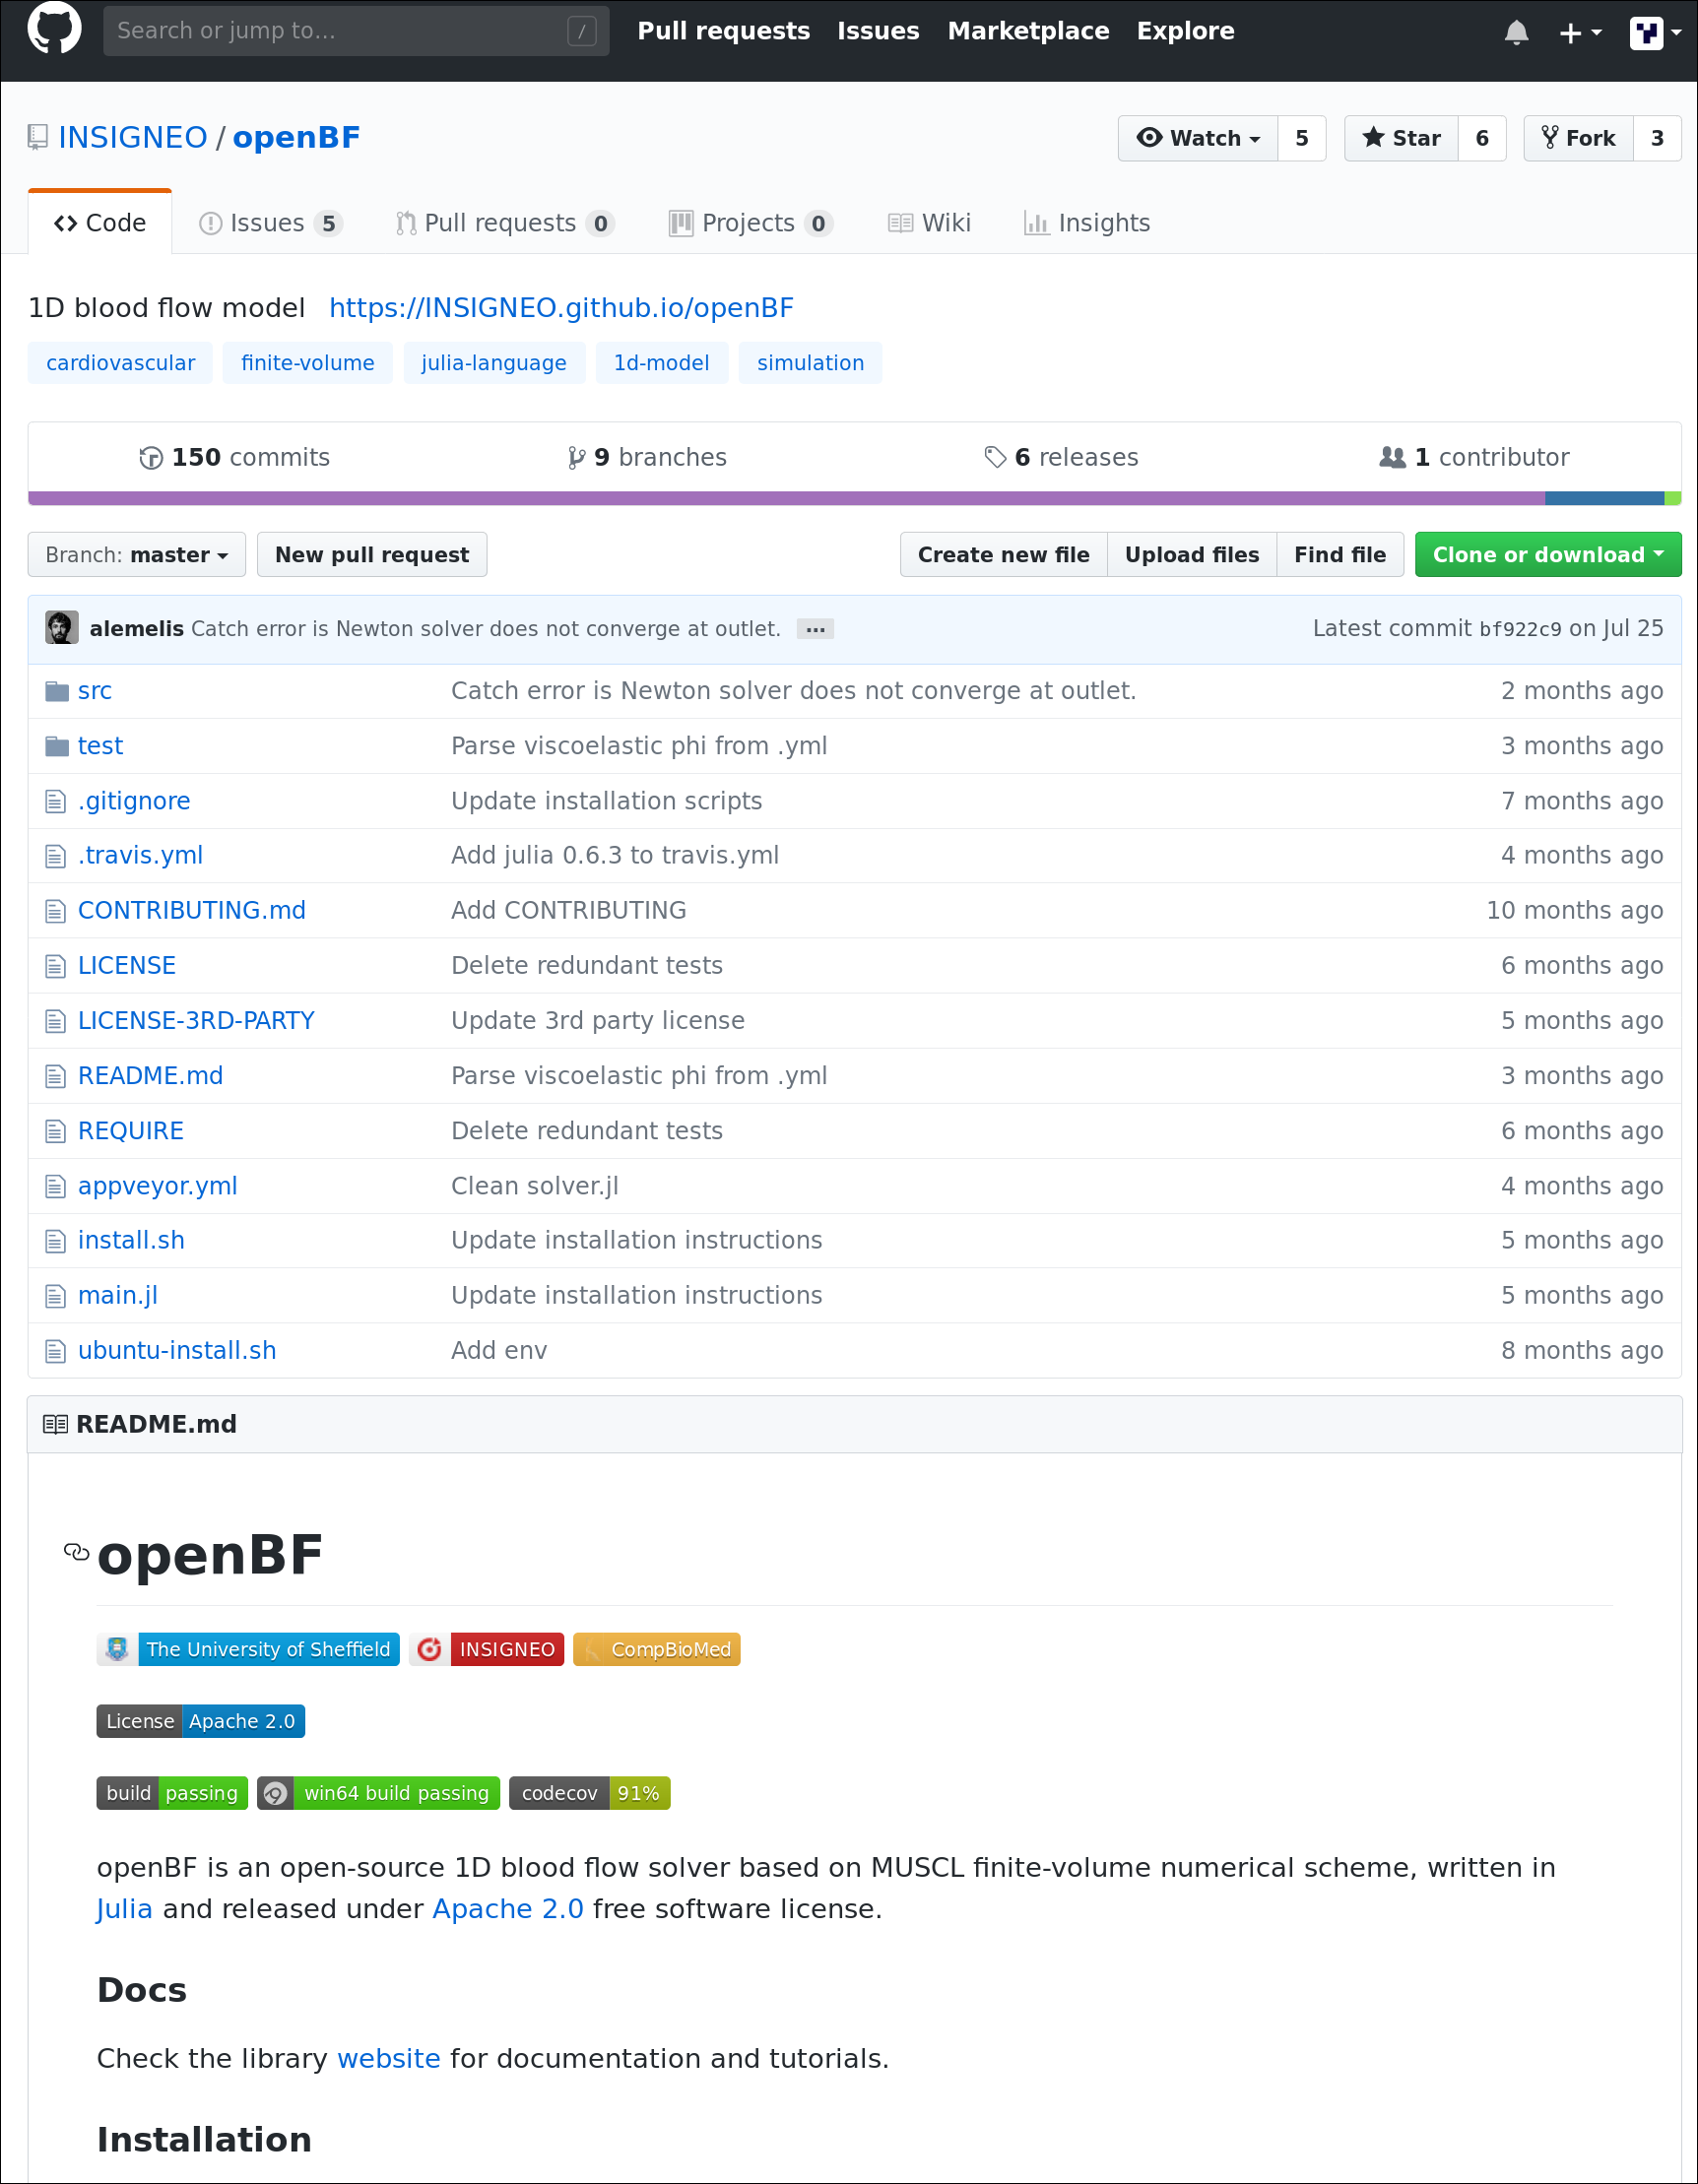
\includegraphics[width=\textwidth]{openbf_gh}
    \end{column}
  \end{columns}
\end{frame}

\begin{frame}
  \frametitle{Testing and Benchmarking}
  \begin{block}{}
    \centering
    
\includegraphics[width=0.4\textwidth]{fixing_problems}
  \end{block}
  \let\thefootnote\relax\footnote{Image Source: Randall Munroe, XKCD (https://xkcd.com/1909/)}
\end{frame}

\begin{frame}
  \frametitle{Testing and Benchmarking}
%  \begin{block}{Testing early and often helps catch mistakes}
    \alert{Testing early and often helps catch mistakes}
    \pause
%    \begin{itemize}
%      \item[] \alert{Ideally test at two different scales:}
    \begin{block}{Ideally test at two different scales:}
        \begin{itemize}
          \item Every function should have accompanying tests (unit tests):
            \begin{itemize}
              \item Ensure functions give correct output for correct input
              \item Graceful failures with invalid input
              \item These should be run every time the code is changed
              \item[]
            \end{itemize}
            \pause
            \item Test full program behaviour (integration tests):
            \begin{itemize}
              \item Identify useful test cases with known results
              \item Test on different machines/architectures
              \item Regression tests: check against previous versions
            \end{itemize}
        \end{itemize}
 %   \end{itemize}
  \end{block}
  \pause
  \alert{Lots of tools to help automate this}
\end{frame}

\begin{frame}
  \frametitle{Testing and Benchmarking}
  \centering
  \begin{block}{Testing Frameworks}
    \begin{itemize}
      \item Tools to automate running of tests
      \item Programmer writes test functions, provides expected output
      \item Framework runs all tests and provides report
    \end{itemize}
  \end{block}
  \vspace{0em}
  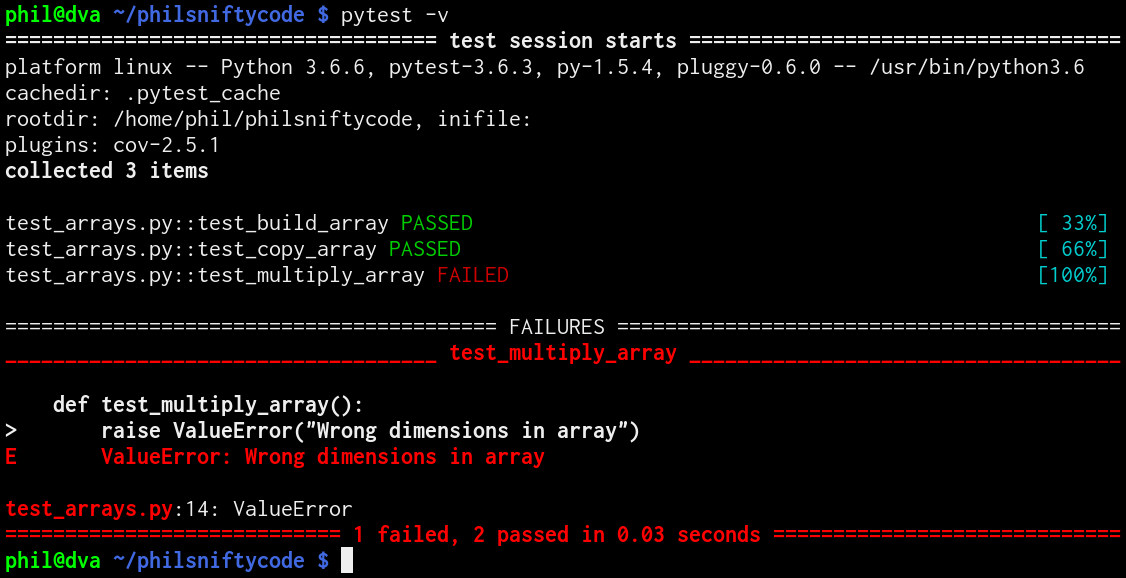
\includegraphics[width=0.7\textwidth]{pytest_example}
\end{frame}

\begin{frame}
  \frametitle{Testing and Benchmarking}
  \centering
  \begin{block}{Continuous Integration}
    \begin{itemize}
      \item Automatically build and test code after changes
      \item Test in different environments (linux/windows), compiler versions
      \item Free services for open source projects
      \item Immediate feedback on bugs/mistakes
    \end{itemize}
  \end{block}
  \vspace{1em}
  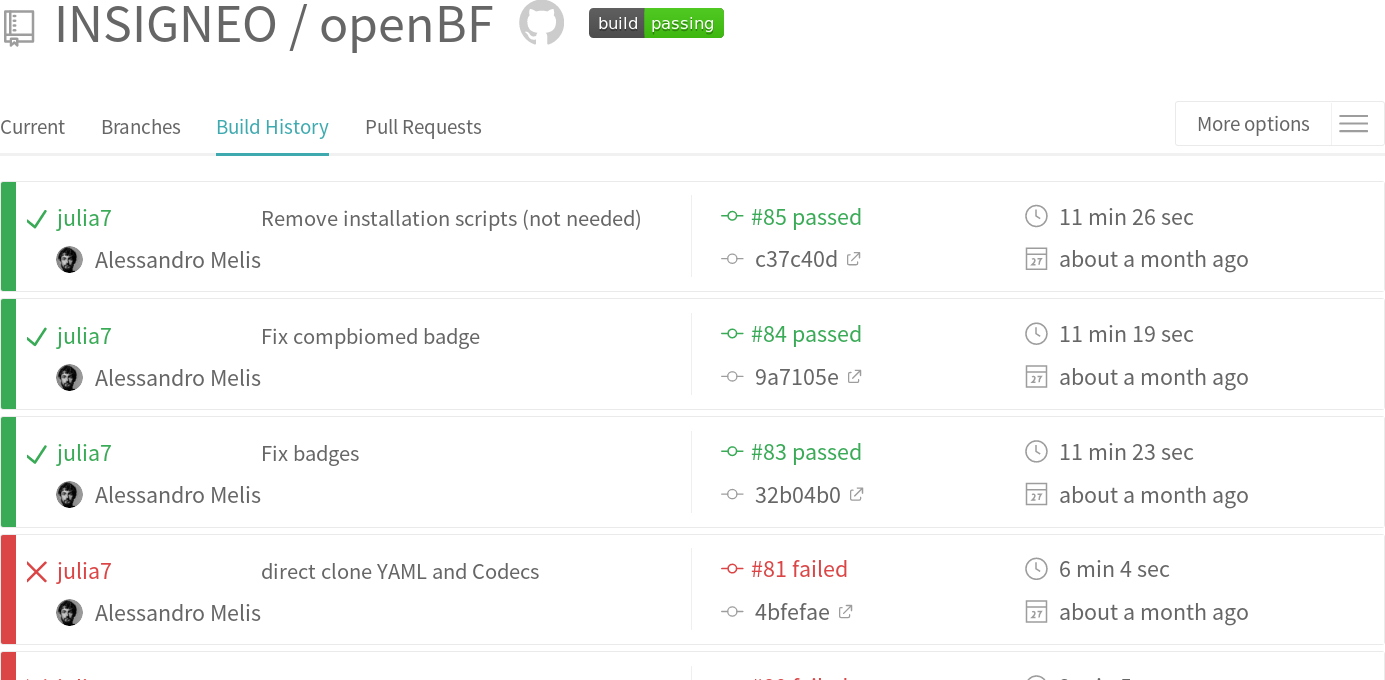
\includegraphics[width=0.7\textwidth]{openbf_travis}
\end{frame}

\begin{frame}
  \frametitle{Documentation}
  \centering
  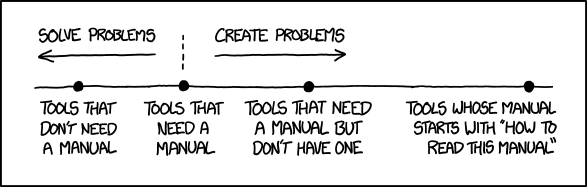
\includegraphics[width=0.7\textwidth]{manuals}
  \let\thefootnote\relax\footnote{Image Source: Randall Munroe, XKCD (https://xkcd.com/1343/)}
\end{frame}


\begin{frame}
  \frametitle{Documentation}
  \centering
  \begin{block}{Getting Users Started}
    \begin{itemize}
      \item Clear installation instructions
      \item Concise tutorial (with example data)
      \item Explanation of output
      \item Troubleshooting?
    \end{itemize}
  \end{block}
\end{frame}

\begin{frame}
  \frametitle{Documentation}
  \centering
  \begin{block}{User Manual}
    \begin{itemize}
      \item Document all features of the program
      \item Details of algorithms and maths used
      \item Advanced usage examples
      \item Test and benchmarking datasets
      \item Known issues, bugs?
    \end{itemize}
  \end{block}
\end{frame}

\begin{frame}
  \frametitle{Documentation}
  \centering
  \begin{block}{API/Internal Documentation}
    \begin{itemize}
      \item Application Programming Interface - functions for your users to call
      \item Document internal functions too
      \item Can be autogenerated from code and comments
      \item Crucial for future developers (you in 5 years?)
    \end{itemize}
  \end{block}
\end{frame}

\begin{frame}
  \frametitle{Documentation}
  \centering
  \begin{block}{Documentation Generators}
    \begin{itemize}
      \item Quickly create professional documentation pages or pdf
      \item Sphinx and Doxygen are most common
      \item Simple human readable format
      \item Build api docs from code and comments
      \item Use with continuous integration - build docs along with your code and host on github
    \end{itemize}
  \end{block}
\end{frame}

\begin{frame}
  \frametitle{Community Building}
  \centering
  \begin{block}{Consumers or Collaborators?}
    \begin{itemize}
      \item Sharing code exposes it to new users and use cases
      \item Bugs \emph{will} be found, encourage reporting
      \item Open source allows users to engage with development
      \item More eyes on code means more issues found and fixed
      \item Contribution of new features
      \item Users help maintain code for you
    \end{itemize}
  \end{block}
  \alert{Platforms like Github provide all this for minimal effort}
\end{frame}

\begin{frame}
  \frametitle{Conclusion: producing good software is hard}
  \centering
  \begin{columns}
    \begin{column}{0.7\textwidth}
      \begin{block}{We all need to:}
        \begin{itemize}
          \item Structure projects carefully
          \item Keep code safe with version control
          \item Backup to Github etc.
          \item Test everything!
          \item[]
          \item Lots of tools available to help
          \item Building a user community shares the burden
          \item Lots of help out there:
            \begin{itemize}
              \item Software Sustainability Institute
              \item Research Software Engineers
              \item Software Carpentry
              \item (Google!)
            \end{itemize}
        \end{itemize}
      \end{block}
    \end{column}
    \begin{column}{0.3\textwidth}
      
\includegraphics[width=0.9\textwidth]{ssi}
      \hfill
      \vspace{1em}
      
\includegraphics[width=0.9\textwidth]{shefrse}
      \hfill
      \vspace{1em}
      
\includegraphics[width=0.9\textwidth]{swcarpentry}
    \end{column}
  \end{columns}
\end{frame}

\begin{frame}
  \frametitle{Useful Resources}
  \begin{itemize}
    \item\alert{Software Sustainability}
    \begin{itemize}
      \item\alert{SSI:} https://software.ac.uk
      \item\alert{Software Carpentry:} https://software-carpentry.org
    \end{itemize}
    \item\alert{Version Control}
    \begin{itemize}
      \item\alert{Github:} https://github.com
      \item\alert{Bitbucket:} https://bitbucket.org
      \item\alert{Git book:} https://git-scm.com/book
    \end{itemize}
  \item\alert{Continuous Integration}
    \begin{itemize}
      \item\alert{Travis:} https://travis-ci.org
      \item\alert{Appveyor:} https://appveyor.com
    \end{itemize}
  \end{itemize}
\end{frame}


\end{document}
